Kiến trúc vi dịch vụ chia dự án thành các thành phần nhỏ hơn được gọi là các dịch vụ.

Mỗi dịch vụ tập trung vào một khả năng kinh doanh cụ thể. 

Các dịch vụ   độc lập và  giao tiếp với nhau thông qua  hạ tầng mạng.


% 
\end{document}

%  và có thể được triển khai, mở rộng quy mô và duy trì độc lập với các dịch vụ khác trong hệ thống. 
  

% Các dịch vụ độc lập về ngôn ngữ lập trình, CSDL, triển khai,...


% Các dịch vụ tương tác với nhau qua hạ tầng mạng.



% \begin{figure}[h]

% \centering

% 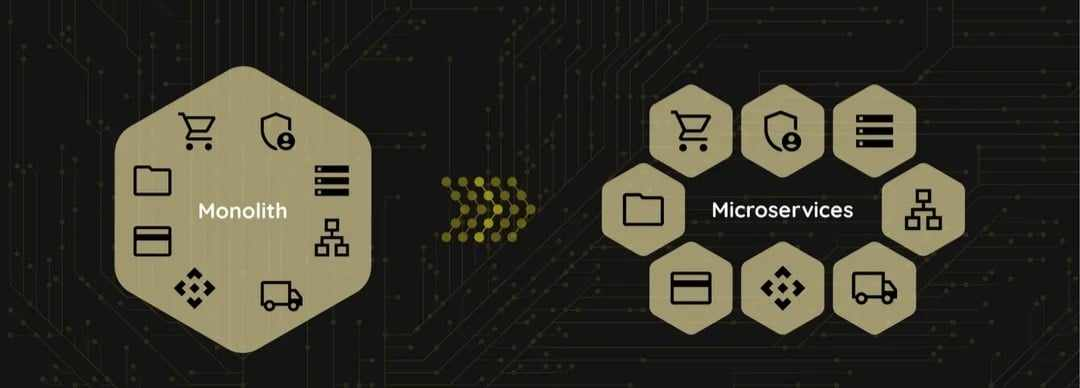
\includegraphics[height = 3cm]{pictures/ChuyenTu_KienTrucNguyenKhoi_Sang_KienTrucViDichVu.jpg}

% % \caption{ViDuHinhAnhTheoChieuDoc}

% \end{figure}

% \begin{figure}[h]

% \centering

% 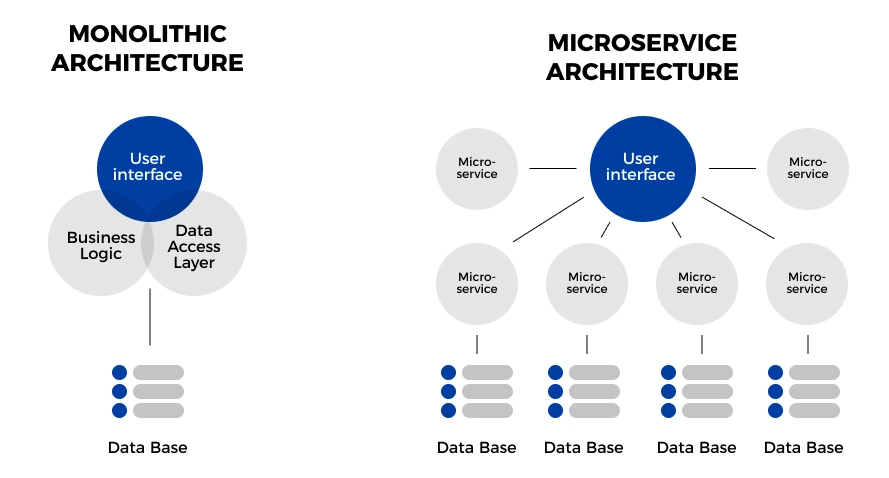
\includegraphics[height = 3cm]{pictures/AnhKhacNhau_KienTrucNguyenKhoi_KienTrucViDichVu.png}

% % \caption{ViDuHinhAnhTheoChieuDoc}

% \end{figure}

% Strangler Fig là chuyển mono sang dịch vụ


